\documentclass[twoside]{book}

% Packages required by doxygen
\usepackage{fixltx2e}
\usepackage{calc}
\usepackage{doxygen}
\usepackage[export]{adjustbox} % also loads graphicx
\usepackage{graphicx}
\usepackage[utf8]{inputenc}
\usepackage{makeidx}
\usepackage{multicol}
\usepackage{multirow}
\PassOptionsToPackage{warn}{textcomp}
\usepackage{textcomp}
\usepackage[nointegrals]{wasysym}
\usepackage[table]{xcolor}

% Font selection
\usepackage[T1]{fontenc}
\usepackage[scaled=.90]{helvet}
\usepackage{courier}
\usepackage{amssymb}
\usepackage{sectsty}
\renewcommand{\familydefault}{\sfdefault}
\allsectionsfont{%
  \fontseries{bc}\selectfont%
  \color{darkgray}%
}
\renewcommand{\DoxyLabelFont}{%
  \fontseries{bc}\selectfont%
  \color{darkgray}%
}
\newcommand{\+}{\discretionary{\mbox{\scriptsize$\hookleftarrow$}}{}{}}

% Page & text layout
\usepackage{geometry}
\geometry{%
  a4paper,%
  top=2.5cm,%
  bottom=2.5cm,%
  left=2.5cm,%
  right=2.5cm%
}
\tolerance=750
\hfuzz=15pt
\hbadness=750
\setlength{\emergencystretch}{15pt}
\setlength{\parindent}{0cm}
\setlength{\parskip}{3ex plus 2ex minus 2ex}
\makeatletter
\renewcommand{\paragraph}{%
  \@startsection{paragraph}{4}{0ex}{-1.0ex}{1.0ex}{%
    \normalfont\normalsize\bfseries\SS@parafont%
  }%
}
\renewcommand{\subparagraph}{%
  \@startsection{subparagraph}{5}{0ex}{-1.0ex}{1.0ex}{%
    \normalfont\normalsize\bfseries\SS@subparafont%
  }%
}
\makeatother

% Headers & footers
\usepackage{fancyhdr}
\pagestyle{fancyplain}
\fancyhead[LE]{\fancyplain{}{\bfseries\thepage}}
\fancyhead[CE]{\fancyplain{}{}}
\fancyhead[RE]{\fancyplain{}{\bfseries\leftmark}}
\fancyhead[LO]{\fancyplain{}{\bfseries\rightmark}}
\fancyhead[CO]{\fancyplain{}{}}
\fancyhead[RO]{\fancyplain{}{\bfseries\thepage}}
\fancyfoot[LE]{\fancyplain{}{}}
\fancyfoot[CE]{\fancyplain{}{}}
\fancyfoot[RE]{\fancyplain{}{\bfseries\scriptsize Generated by Doxygen }}
\fancyfoot[LO]{\fancyplain{}{\bfseries\scriptsize Generated by Doxygen }}
\fancyfoot[CO]{\fancyplain{}{}}
\fancyfoot[RO]{\fancyplain{}{}}
\renewcommand{\footrulewidth}{0.4pt}
\renewcommand{\chaptermark}[1]{%
  \markboth{#1}{}%
}
\renewcommand{\sectionmark}[1]{%
  \markright{\thesection\ #1}%
}

% Indices & bibliography
\usepackage{natbib}
\usepackage[titles]{tocloft}
\setcounter{tocdepth}{3}
\setcounter{secnumdepth}{5}
\makeindex

% Hyperlinks (required, but should be loaded last)
\usepackage{ifpdf}
\ifpdf
  \usepackage[pdftex,pagebackref=true]{hyperref}
\else
  \usepackage[ps2pdf,pagebackref=true]{hyperref}
\fi
\hypersetup{%
  colorlinks=true,%
  linkcolor=blue,%
  citecolor=blue,%
  unicode%
}

% Custom commands
\newcommand{\clearemptydoublepage}{%
  \newpage{\pagestyle{empty}\cleardoublepage}%
}

\usepackage{caption}
\captionsetup{labelsep=space,justification=centering,font={bf},singlelinecheck=off,skip=4pt,position=top}

%===== C O N T E N T S =====

\begin{document}

% Titlepage & ToC
\hypersetup{pageanchor=false,
             bookmarksnumbered=true,
             pdfencoding=unicode
            }
\pagenumbering{alph}
\begin{titlepage}
\vspace*{7cm}
\begin{center}%
{\Large Lab 8 }\\
\vspace*{1cm}
{\large Generated by Doxygen 1.8.13}\\
\end{center}
\end{titlepage}
\clearemptydoublepage
\pagenumbering{roman}
\tableofcontents
\clearemptydoublepage
\pagenumbering{arabic}
\hypersetup{pageanchor=true}

%--- Begin generated contents ---
\chapter{Class Index}
\section{Class List}
Here are the classes, structs, unions and interfaces with brief descriptions\+:\begin{DoxyCompactList}
\item\contentsline{section}{\hyperlink{classActor}{Actor} }{\pageref{classActor}}{}
\item\contentsline{section}{\hyperlink{classActorsLoader}{Actors\+Loader} }{\pageref{classActorsLoader}}{}
\item\contentsline{section}{\hyperlink{structRequest}{Request} \\*Struct, whitch used in privates methods of class \hyperlink{classServer}{Server} to get type of request }{\pageref{structRequest}}{}
\item\contentsline{section}{\hyperlink{classServer}{Server} }{\pageref{classServer}}{}
\end{DoxyCompactList}

\chapter{File Index}
\section{File List}
Here is a list of all documented files with brief descriptions\+:\begin{DoxyCompactList}
\item\contentsline{section}{include/\hyperlink{actor_8h}{actor.\+h} \\*Class \hyperlink{classActor}{Actor} }{\pageref{actor_8h}}{}
\item\contentsline{section}{include/\hyperlink{actorsLoader_8h}{actors\+Loader.\+h} \\*Class to get actors information from Im\+DB A\+PI }{\pageref{actorsLoader_8h}}{}
\item\contentsline{section}{include/\hyperlink{server_8h}{server.\+h} \\*\hyperlink{classServer}{Server} class }{\pageref{server_8h}}{}
\end{DoxyCompactList}

\chapter{Class Documentation}
\hypertarget{classActor}{}\section{Actor Class Reference}
\label{classActor}\index{Actor@{Actor}}
\subsection*{Public Member Functions}
\begin{DoxyCompactItemize}
\item 
\mbox{\Hypertarget{classActor_a3e39141bcd920c816e08bdfafe3f73d5}\label{classActor_a3e39141bcd920c816e08bdfafe3f73d5}} 
\hyperlink{classActor_a3e39141bcd920c816e08bdfafe3f73d5}{Actor} (std\+::string \hyperlink{classActor_aeefa8310b4b62d376c69b3ef080f13d4}{id}, std\+::string full\+Name, std\+::string film)
\begin{DoxyCompactList}\small\item\em \hyperlink{classActor}{Actor} constructor. \end{DoxyCompactList}\item 
std\+::string \hyperlink{classActor_aeefa8310b4b62d376c69b3ef080f13d4}{id} ()
\begin{DoxyCompactList}\small\item\em getting id on Im\+DB of actor \end{DoxyCompactList}\item 
std\+::string \hyperlink{classActor_a9c6aa7e7cd5e8183ea66aa97eb6b015c}{name} ()
\begin{DoxyCompactList}\small\item\em getting name of actor \end{DoxyCompactList}\item 
std\+::string \hyperlink{classActor_a0cf1e28725cadacefb040914667cd5cc}{surname} ()
\begin{DoxyCompactList}\small\item\em getting surname actor \end{DoxyCompactList}\item 
std\+::string \hyperlink{classActor_a26e7eb5386554b5f35e91e55aca633c3}{most\+Popular\+Film} ()
\begin{DoxyCompactList}\small\item\em getting most popular film with actor \end{DoxyCompactList}\end{DoxyCompactItemize}


\subsection{Member Function Documentation}
\mbox{\Hypertarget{classActor_aeefa8310b4b62d376c69b3ef080f13d4}\label{classActor_aeefa8310b4b62d376c69b3ef080f13d4}} 
\index{Actor@{Actor}!id@{id}}
\index{id@{id}!Actor@{Actor}}
\subsubsection{\texorpdfstring{id()}{id()}}
{\footnotesize\ttfamily std\+::string Actor\+::id (\begin{DoxyParamCaption}{ }\end{DoxyParamCaption})}



getting id on Im\+DB of actor 

\begin{DoxyReturn}{Returns}
string with id 
\end{DoxyReturn}
\mbox{\Hypertarget{classActor_a26e7eb5386554b5f35e91e55aca633c3}\label{classActor_a26e7eb5386554b5f35e91e55aca633c3}} 
\index{Actor@{Actor}!most\+Popular\+Film@{most\+Popular\+Film}}
\index{most\+Popular\+Film@{most\+Popular\+Film}!Actor@{Actor}}
\subsubsection{\texorpdfstring{most\+Popular\+Film()}{mostPopularFilm()}}
{\footnotesize\ttfamily std\+::string Actor\+::most\+Popular\+Film (\begin{DoxyParamCaption}{ }\end{DoxyParamCaption})}



getting most popular film with actor 

\begin{DoxyReturn}{Returns}
string with most popular film 
\end{DoxyReturn}
\mbox{\Hypertarget{classActor_a9c6aa7e7cd5e8183ea66aa97eb6b015c}\label{classActor_a9c6aa7e7cd5e8183ea66aa97eb6b015c}} 
\index{Actor@{Actor}!name@{name}}
\index{name@{name}!Actor@{Actor}}
\subsubsection{\texorpdfstring{name()}{name()}}
{\footnotesize\ttfamily std\+::string Actor\+::name (\begin{DoxyParamCaption}{ }\end{DoxyParamCaption})}



getting name of actor 

\begin{DoxyReturn}{Returns}
string with name 
\end{DoxyReturn}
\mbox{\Hypertarget{classActor_a0cf1e28725cadacefb040914667cd5cc}\label{classActor_a0cf1e28725cadacefb040914667cd5cc}} 
\index{Actor@{Actor}!surname@{surname}}
\index{surname@{surname}!Actor@{Actor}}
\subsubsection{\texorpdfstring{surname()}{surname()}}
{\footnotesize\ttfamily std\+::string Actor\+::surname (\begin{DoxyParamCaption}{ }\end{DoxyParamCaption})}



getting surname actor 

\begin{DoxyReturn}{Returns}
string with surname 
\end{DoxyReturn}


The documentation for this class was generated from the following files\+:\begin{DoxyCompactItemize}
\item 
include/\hyperlink{actor_8h}{actor.\+h}\item 
src/actor.\+cpp\end{DoxyCompactItemize}

\hypertarget{classActorsLoader}{}\section{Actors\+Loader Class Reference}
\label{classActorsLoader}\index{Actors\+Loader@{Actors\+Loader}}
\subsection*{Public Member Functions}
\begin{DoxyCompactItemize}
\item 
\mbox{\Hypertarget{classActorsLoader_a130deecc6b389e7dfe1a1ee6a4b0ab9f}\label{classActorsLoader_a130deecc6b389e7dfe1a1ee6a4b0ab9f}} 
\hyperlink{classActorsLoader_a130deecc6b389e7dfe1a1ee6a4b0ab9f}{Actors\+Loader} ()
\begin{DoxyCompactList}\small\item\em \hyperlink{classActorsLoader}{Actors\+Loader} constructor. \end{DoxyCompactList}\item 
\mbox{\Hypertarget{classActorsLoader_a36b062dd3ec38eb064570972b60bf0e7}\label{classActorsLoader_a36b062dd3ec38eb064570972b60bf0e7}} 
\hyperlink{classActorsLoader_a36b062dd3ec38eb064570972b60bf0e7}{$\sim$\+Actors\+Loader} ()
\begin{DoxyCompactList}\small\item\em \hyperlink{classActorsLoader}{Actors\+Loader} destructor. \end{DoxyCompactList}\item 
\mbox{\Hypertarget{classActorsLoader_af6cd0bc5b9b13e194f419564bca8f082}\label{classActorsLoader_af6cd0bc5b9b13e194f419564bca8f082}} 
void \hyperlink{classActorsLoader_af6cd0bc5b9b13e194f419564bca8f082}{connect\+To\+I\+M\+DB} ()
\begin{DoxyCompactList}\small\item\em connecting to Im\+DB A\+PI \end{DoxyCompactList}\item 
std\+::list$<$ \hyperlink{classActor}{Actor} $\ast$ $>$ \hyperlink{classActorsLoader_a874dc64afbddc3d49182139c6f3c2510}{get\+List\+Of\+Actors} ()
\begin{DoxyCompactList}\small\item\em getting list of actors \end{DoxyCompactList}\end{DoxyCompactItemize}


\subsection{Member Function Documentation}
\mbox{\Hypertarget{classActorsLoader_a874dc64afbddc3d49182139c6f3c2510}\label{classActorsLoader_a874dc64afbddc3d49182139c6f3c2510}} 
\index{Actors\+Loader@{Actors\+Loader}!get\+List\+Of\+Actors@{get\+List\+Of\+Actors}}
\index{get\+List\+Of\+Actors@{get\+List\+Of\+Actors}!Actors\+Loader@{Actors\+Loader}}
\subsubsection{\texorpdfstring{get\+List\+Of\+Actors()}{getListOfActors()}}
{\footnotesize\ttfamily std\+::list$<$ \hyperlink{classActor}{Actor} $\ast$ $>$ Actors\+Loader\+::get\+List\+Of\+Actors (\begin{DoxyParamCaption}{ }\end{DoxyParamCaption})}



getting list of actors 

\begin{DoxyReturn}{Returns}
list of actors 
\end{DoxyReturn}


The documentation for this class was generated from the following files\+:\begin{DoxyCompactItemize}
\item 
include/\hyperlink{actorsLoader_8h}{actors\+Loader.\+h}\item 
src/actors\+Loader.\+cpp\end{DoxyCompactItemize}

\hypertarget{structRequest}{}\section{Request Struct Reference}
\label{structRequest}\index{Request@{Request}}


struct, whitch used in privates methods of class \hyperlink{classServer}{Server} to get type of request  




{\ttfamily \#include $<$server.\+h$>$}

\subsection*{Public Attributes}
\begin{DoxyCompactItemize}
\item 
\mbox{\Hypertarget{structRequest_affc001ac329251d9015065c5643cae67}\label{structRequest_affc001ac329251d9015065c5643cae67}} 
Request\+Type {\bfseries type}
\item 
\mbox{\Hypertarget{structRequest_ae844057c9d9aa9fc3a7e762a3a7e1960}\label{structRequest_ae844057c9d9aa9fc3a7e762a3a7e1960}} 
std\+::string {\bfseries key}
\item 
\mbox{\Hypertarget{structRequest_a1a1a4e754b5081515d668e2ab8060d4a}\label{structRequest_a1a1a4e754b5081515d668e2ab8060d4a}} 
std\+::string {\bfseries value}
\item 
\mbox{\Hypertarget{structRequest_a026538b5d27774177b27d0552d25fa13}\label{structRequest_a026538b5d27774177b27d0552d25fa13}} 
int {\bfseries id}
\end{DoxyCompactItemize}


\subsection{Detailed Description}
struct, whitch used in privates methods of class \hyperlink{classServer}{Server} to get type of request 

The documentation for this struct was generated from the following file\+:\begin{DoxyCompactItemize}
\item 
src/server.\+cpp\end{DoxyCompactItemize}

\hypertarget{classServer}{}\section{Server Class Reference}
\label{classServer}\index{Server@{Server}}
\subsection*{Public Member Functions}
\begin{DoxyCompactItemize}
\item 
\mbox{\Hypertarget{classServer_a7d1fe6ba5f0fe9190a4f039662ea0e85}\label{classServer_a7d1fe6ba5f0fe9190a4f039662ea0e85}} 
\hyperlink{classServer_a7d1fe6ba5f0fe9190a4f039662ea0e85}{Server} (int port)
\begin{DoxyCompactList}\small\item\em \hyperlink{classServer}{Server} construction. \end{DoxyCompactList}\item 
\mbox{\Hypertarget{classServer_a4b3aa2579cb1c8cd1d069582c14d0fa6}\label{classServer_a4b3aa2579cb1c8cd1d069582c14d0fa6}} 
\hyperlink{classServer_a4b3aa2579cb1c8cd1d069582c14d0fa6}{$\sim$\+Server} ()
\begin{DoxyCompactList}\small\item\em \hyperlink{classServer}{Server} destructor. \end{DoxyCompactList}\item 
\mbox{\Hypertarget{classServer_a0e4dd73ec8cef85f5145e286cf9cd3dc}\label{classServer_a0e4dd73ec8cef85f5145e286cf9cd3dc}} 
void \hyperlink{classServer_a0e4dd73ec8cef85f5145e286cf9cd3dc}{work} ()
\begin{DoxyCompactList}\small\item\em starting of server and handling clients \end{DoxyCompactList}\end{DoxyCompactItemize}


The documentation for this class was generated from the following files\+:\begin{DoxyCompactItemize}
\item 
include/\hyperlink{server_8h}{server.\+h}\item 
src/server.\+cpp\end{DoxyCompactItemize}

\chapter{File Documentation}
\hypertarget{actor_8h}{}\section{include/actor.h File Reference}
\label{actor_8h}\index{include/actor.\+h@{include/actor.\+h}}


class \hyperlink{classActor}{Actor}  


{\ttfamily \#include $<$string$>$}\newline
Include dependency graph for actor.\+h\+:\nopagebreak
\begin{figure}[H]
\begin{center}
\leavevmode
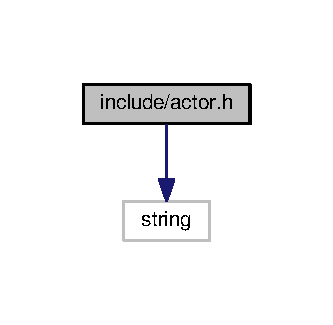
\includegraphics[width=160pt]{actor_8h__incl}
\end{center}
\end{figure}
This graph shows which files directly or indirectly include this file\+:\nopagebreak
\begin{figure}[H]
\begin{center}
\leavevmode
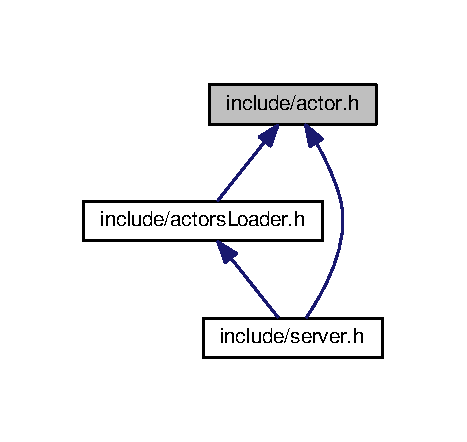
\includegraphics[width=224pt]{actor_8h__dep__incl}
\end{center}
\end{figure}
\subsection*{Classes}
\begin{DoxyCompactItemize}
\item 
class \hyperlink{classActor}{Actor}
\end{DoxyCompactItemize}


\subsection{Detailed Description}
class \hyperlink{classActor}{Actor} 


\hypertarget{actorsLoader_8h}{}\section{include/actors\+Loader.h File Reference}
\label{actorsLoader_8h}\index{include/actors\+Loader.\+h@{include/actors\+Loader.\+h}}


class to get actors information from Im\+DB A\+PI  


{\ttfamily \#include $<$progbase-\/cpp/net.\+h$>$}\newline
{\ttfamily \#include \char`\"{}actor.\+h\char`\"{}}\newline
{\ttfamily \#include $<$list$>$}\newline
Include dependency graph for actors\+Loader.\+h\+:\nopagebreak
\begin{figure}[H]
\begin{center}
\leavevmode
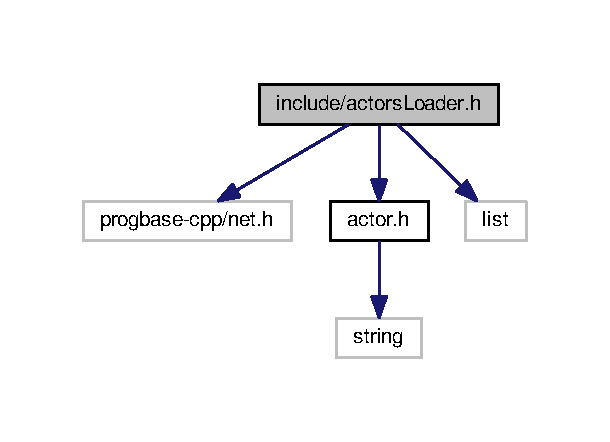
\includegraphics[width=293pt]{actorsLoader_8h__incl}
\end{center}
\end{figure}
This graph shows which files directly or indirectly include this file\+:\nopagebreak
\begin{figure}[H]
\begin{center}
\leavevmode
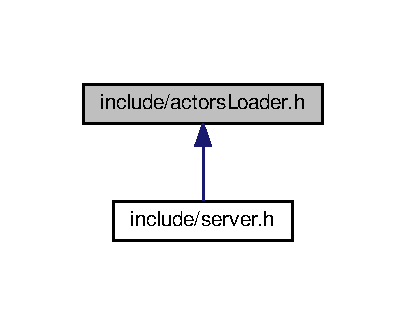
\includegraphics[width=195pt]{actorsLoader_8h__dep__incl}
\end{center}
\end{figure}
\subsection*{Classes}
\begin{DoxyCompactItemize}
\item 
class \hyperlink{classActorsLoader}{Actors\+Loader}
\end{DoxyCompactItemize}


\subsection{Detailed Description}
class to get actors information from Im\+DB A\+PI 


\hypertarget{server_8h}{}\section{include/server.h File Reference}
\label{server_8h}\index{include/server.\+h@{include/server.\+h}}


\hyperlink{classServer}{Server} class.  


{\ttfamily \#include $<$progbase-\/cpp/net.\+h$>$}\newline
{\ttfamily \#include \char`\"{}actors\+Loader.\+h\char`\"{}}\newline
{\ttfamily \#include \char`\"{}actor.\+h\char`\"{}}\newline
Include dependency graph for server.\+h\+:\nopagebreak
\begin{figure}[H]
\begin{center}
\leavevmode
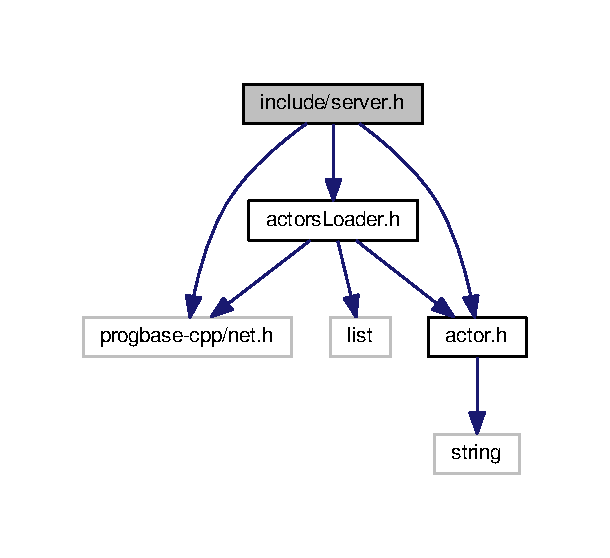
\includegraphics[width=293pt]{server_8h__incl}
\end{center}
\end{figure}
\subsection*{Classes}
\begin{DoxyCompactItemize}
\item 
class \hyperlink{classServer}{Server}
\end{DoxyCompactItemize}


\subsection{Detailed Description}
\hyperlink{classServer}{Server} class. 


%--- End generated contents ---

% Index
\backmatter
\newpage
\phantomsection
\clearemptydoublepage
\addcontentsline{toc}{chapter}{Index}
\printindex

\end{document}
